%%%%%%% Functions
\documentclass[tikz]{standalone}
\usepackage{tikz}
\usepackage{pstricks}
\usepackage[mathrm,colour,cntbysection]{czt}
\usetikzlibrary{calc,trees,positioning,arrows,chains,shapes.geometric,%
	shapes,shadows,matrix,snakes ,fit,calc}

\pgfdeclarelayer{background}
\pgfsetlayers{background,main}


\definecolor{mygray}{gray}{0.3}
\definecolor{lightgray}{gray}{0.6}

\begin{document}
	%%relation page 1
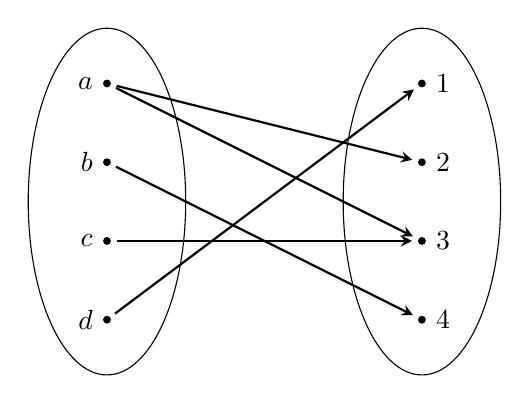
\begin{tikzpicture}[
>=stealth,
bullet/.style={
	fill=black,
	circle,
	minimum width=1pt,
	inner sep=1pt
},
projection/.style={
	->,
	thick,
	shorten <=2pt,
	shorten >=2pt
},
every fit/.style={
	ellipse,
	draw,
	inner sep=0pt
}
]
\foreach \y/\l in {1/d,2/c/,3/b,4/a}
\node[bullet,label=left:$\l$] (a\y) at (0,\y) {};

\foreach \y/\l in {1/4,2/3,3/2,4/1}
\node[bullet,label=right:$\l$] (b\y) at (4,\y) {};

\node[draw,fit=(a1) (a2) (a3) (a4),minimum width=2cm] {} ;
\node[draw,fit=(b1) (b2) (b3) (b4),minimum width=2cm] {} ;

\draw[projection] (a1) -- (b4);
\draw[projection] (a4) -- (b2);
\draw[projection] (a2) -- (b2);
\draw[projection] (a3) -- (b1);
\draw[projection] (a4) -- (b3);
\end{tikzpicture}
%function page 2
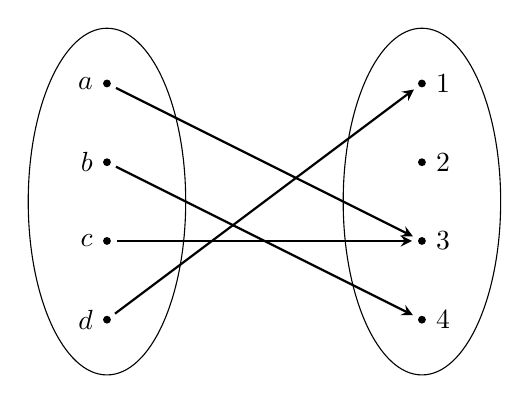
\begin{tikzpicture}[
>=stealth,
bullet/.style={
	fill=black,
	circle,
	minimum width=1pt,
	inner sep=1pt
},
projection/.style={
	->,
	thick,
	shorten <=2pt,
	shorten >=2pt
},
every fit/.style={
	ellipse,
	draw,
	inner sep=0pt
}
]
\foreach \y/\l in {1/d,2/c/,3/b,4/a}
\node[bullet,label=left:$\l$] (a\y) at (0,\y) {};

\foreach \y/\l in {1/4,2/3,3/2,4/1}
\node[bullet,label=right:$\l$] (b\y) at (4,\y) {};

\node[draw,fit=(a1) (a2) (a3) (a4),minimum width=2cm] {} ;
\node[draw,fit=(b1) (b2) (b3) (b4),minimum width=2cm] {} ;

\draw[projection] (a1) -- (b4);
\draw[projection] (a4) -- (b2);
\draw[projection] (a2) -- (b2);
\draw[projection] (a3) -- (b1);
%\draw[projection] (a4) -- (b3);
\end{tikzpicture}
%%Function application page 3
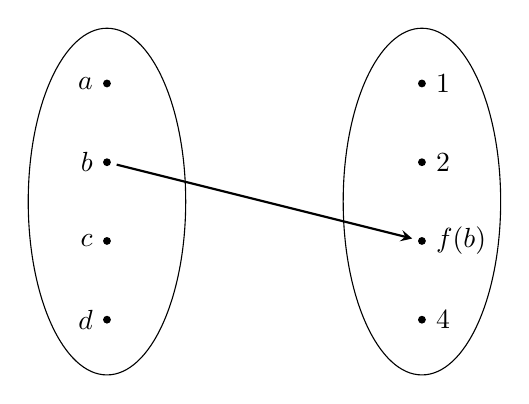
\begin{tikzpicture}[
>=stealth,
bullet/.style={
	fill=black,
	circle,
	minimum width=1pt,
	inner sep=1pt
},
projection/.style={
	->,
	thick,
	shorten <=2pt,
	shorten >=2pt
},
every fit/.style={
	ellipse,
	draw,
	inner sep=0pt
}
]
\foreach \y/\l in {1/d,2/c/,3/b,4/a}
\node[bullet,label=left:$\l$] (a\y) at (0,\y) {};

\foreach \y/\l in {1/4,2/f(b),3/2,4/1}
\node[bullet,label=right:$\l$] (b\y) at (4,\y) {};

\node[draw,fit=(a1) (a2) (a3) (a4),minimum width=2cm] {} ;
\node[draw,fit=(b1) (b2) (b3) (b4),minimum width=2cm] {} ;

%\draw[projection] (a1) -- (b4);
%\draw[projection] (a4) -- (b2);
%\draw[projection] (a2) -- (b2);
\draw[projection] (a3) -- (b2);
%\draw[projection] (a4) -- (b3);
\end{tikzpicture}

% pic of injection
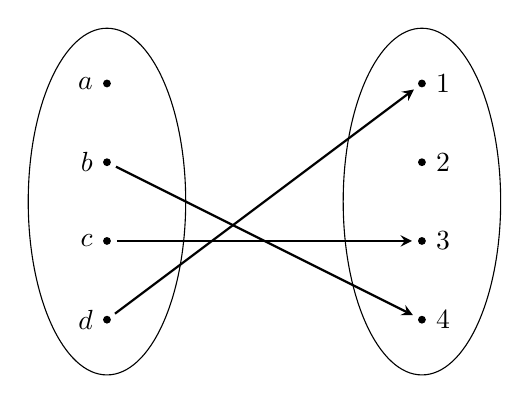
\begin{tikzpicture}[
>=stealth,
bullet/.style={
	fill=black,
	circle,
	minimum width=1pt,
	inner sep=1pt
},
projection/.style={
	->,
	thick,
	shorten <=2pt,
	shorten >=2pt
},
every fit/.style={
	ellipse,
	draw,
	inner sep=0pt
}
]
\foreach \y/\l in {1/d,2/c/,3/b,4/a}
\node[bullet,label=left:$\l$] (a\y) at (0,\y) {};

\foreach \y/\l in {1/4,2/3,3/2,4/1}
\node[bullet,label=right:$\l$] (b\y) at (4,\y) {};

\node[draw,fit=(a1) (a2) (a3) (a4),minimum width=2cm] {} ;
\node[draw,fit=(b1) (b2) (b3) (b4),minimum width=2cm] {} ;

\draw[projection] (a1) -- (b4);
%\draw[projection] (a4) -- (b2);
\draw[projection] (a2) -- (b2);
\draw[projection] (a3) -- (b1);
%\draw[projection] (a4) -- (b3);
\end{tikzpicture}

% pic of partial function
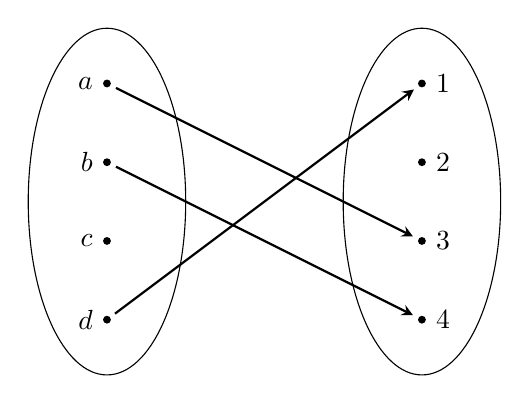
\begin{tikzpicture}[
>=stealth,
bullet/.style={
	fill=black,
	circle,
	minimum width=1pt,
	inner sep=1pt
},
projection/.style={
	->,
	thick,
	shorten <=2pt,
	shorten >=2pt
},
every fit/.style={
	ellipse,
	draw,
	inner sep=0pt
}
]
\foreach \y/\l in {1/d,2/c/,3/b,4/a}
\node[bullet,label=left:$\l$] (a\y) at (0,\y) {};

\foreach \y/\l in {1/4,2/3,3/2,4/1}
\node[bullet,label=right:$\l$] (b\y) at (4,\y) {};

\node[draw,fit=(a1) (a2) (a3) (a4),minimum width=2cm] {} ;
\node[draw,fit=(b1) (b2) (b3) (b4),minimum width=2cm] {} ;

\draw[projection] (a1) -- (b4);
\draw[projection] (a4) -- (b2);
%\draw[projection] (a2) -- (b2);
\draw[projection] (a3) -- (b1);
\end{tikzpicture}


% pic of total function
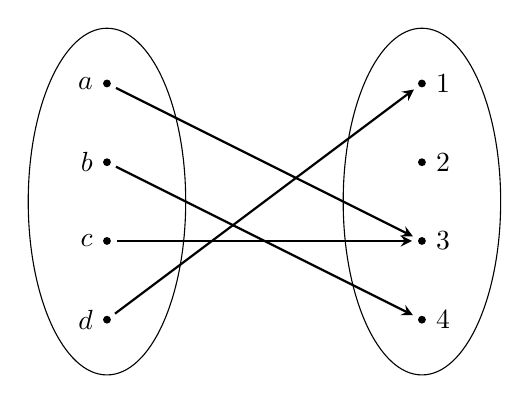
\begin{tikzpicture}[
>=stealth,
bullet/.style={
	fill=black,
	circle,
	minimum width=1pt,
	inner sep=1pt
},
projection/.style={
	->,
	thick,
	shorten <=2pt,
	shorten >=2pt
},
every fit/.style={
	ellipse,
	draw,
	inner sep=0pt
}
]
\foreach \y/\l in {1/d,2/c/,3/b,4/a}
\node[bullet,label=left:$\l$] (a\y) at (0,\y) {};

\foreach \y/\l in {1/4,2/3,3/2,4/1}
\node[bullet,label=right:$\l$] (b\y) at (4,\y) {};

\node[draw,fit=(a1) (a2) (a3) (a4),minimum width=2cm] {} ;
\node[draw,fit=(b1) (b2) (b3) (b4),minimum width=2cm] {} ;

\draw[projection] (a1) -- (b4);
\draw[projection] (a4) -- (b2);
\draw[projection] (a2) -- (b2);
\draw[projection] (a3) -- (b1);
%\draw[projection] (a4) -- (b3);
\end{tikzpicture}

% pic of surrjective  function
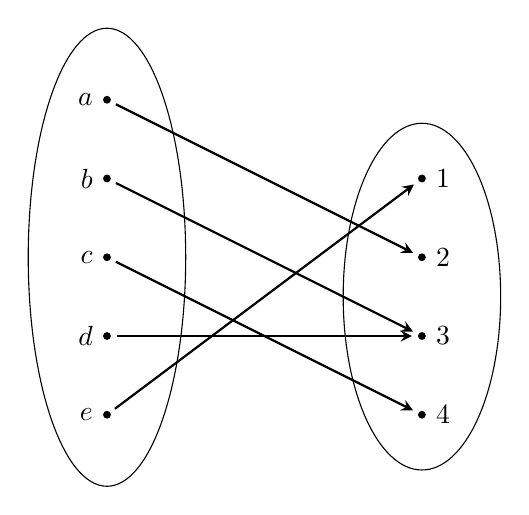
\begin{tikzpicture}[
>=stealth,
bullet/.style={
	fill=black,
	circle,
	minimum width=1pt,
	inner sep=1pt
},
projection/.style={
	->,
	thick,
	shorten <=2pt,
	shorten >=2pt
},
every fit/.style={
	ellipse,
	draw,
	inner sep=0pt
}
]
\foreach \y/\l in {1/e, 2/d,3/c/,4/b,5/a}
\node[bullet,label=left:$\l$] (a\y) at (0,\y) {};

\foreach \y/\l in {1/4,2/3,3/2,4/1}
\node[bullet,label=right:$\l$] (b\y) at (4,\y) {};

\node[draw,fit=(a1) (a2) (a3) (a4) (a5) ,minimum width=2cm] {} ;
\node[draw,fit=(b1) (b2) (b3) (b4),minimum width=2cm] {} ;

\draw[projection] (a1) -- (b4);
\draw[projection] (a4) -- (b2);
\draw[projection] (a2) -- (b2);
\draw[projection] (a3) -- (b1);
\draw[projection] (a5) -- (b3);
\end{tikzpicture}

\end{document}